
\info{
	on rappelle les notations suivantes :

	\begin{itemize}
		\item vrai : $\theta = \mathds E \bigl[ \, f(X) \, \bigr]$
		\item intangible : $\widetilde \theta = \frac 1 N \sum_i f(X_i)$
		\item observable : $\hat \theta = \frac 1 N \sum_i f(\widehat X_i)$
	\end{itemize}
}

L'estimateur du paramètre de régularité $H_t$ est donné par :

$$\hat H_t = \frac{ \log \hat \theta(t_1, t_3) - \log \hat \theta(t_1, t_2) }{2 \log 2}$$

ou bien encore :

$$\hat H_t = \frac{ \log \hat \theta(t_1, t_3) - \log \hat \theta(t_2, t_3) }{2 \log 2}$$


autrement dit :

en posant
\begin{minipage}{0.5\textwidth}
	\begin{equation*}
		\thetaA = \begin{bmatrix} \theta(t_1, t_3) \\ \theta(t_1, t_2) \end{bmatrix}
	\end{equation*}
\end{minipage}
\hfill
\begin{minipage}{0.5\textwidth}
	\begin{equation*}
		\thetaB = \begin{bmatrix} \theta(t_1, t_3) \\ \theta(t_2, t_3) \end{bmatrix}
	\end{equation*}
\end{minipage}

\smallskip

L'estimateur du paramètre de régularité $H_t$ peut se ré-écrire comme :

\smallskip


\begin{equation*}
	\widehat H_t : \Theta \longmapsto \frac{ \log \widehat \Theta_1 - \log \widehat \Theta_2 }{2 \log 2}
\end{equation*}

\smallskip

C'est pourquoi, étant donné que le meilleur estimateur que l'on puisse espérer soit $\bigl(\hat H_t( \widetilde \thetaA)$ ou $\hat H_t( \widetilde \thetaB)\bigr)$, on va s'intéresser désormais à l'estimation conjointe des deux $\theta(u,v)$ utilisés dans l'estimation de $H_t$ comme critère de sélection du diamètre $\Delta$.

\begin{figure}[H]
	\centering
	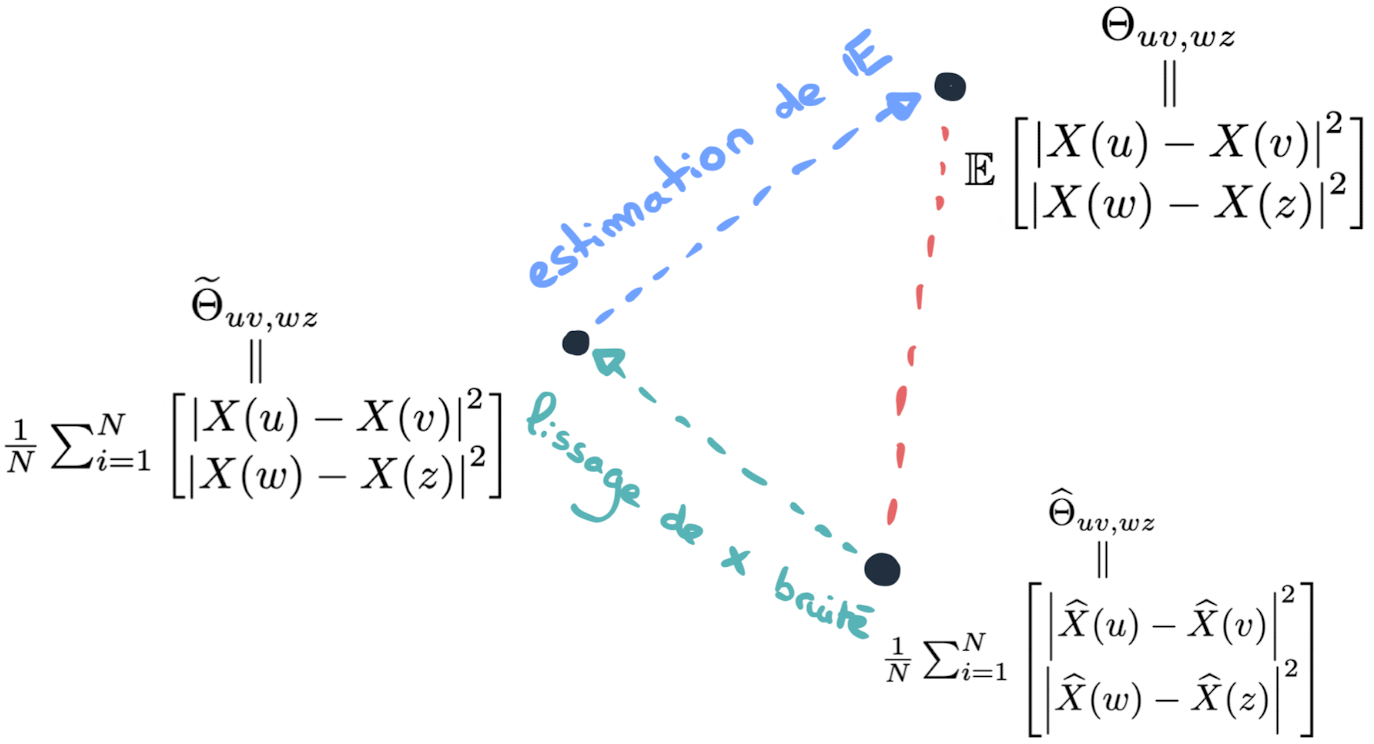
\includegraphics[width=0.7\textwidth]{Images/sketches/theta_biais.png}
	\caption{Schéma représentant les différents biais et approximations du couple d'incréments}
	\label{fig:sketch_theta_biais}
\end{figure}


Pour cela on considère la distance euclidienne usuelle pour des vecteurs de $\R 2$

$$R(\Theta, \Delta) = \distnorme 2 {\widehat \Theta(\Delta)} {\widetilde \Theta(\Delta)}$$

et on nomme $R\cindexA(\Delta) = R( \thetaA , \, \Delta \, )$ et $R\cindexB(\Delta) = R( \thetaB, \, \Delta \, )$

\begin{table}[H]
	\centering
	\begin{tabular}{l|ll|}
		\cline{2-3}
		                                     & $\lambda < 120$                                                                                                                                                                                                           & $\lambda \geq 120$                                                                             \\ \hline
		\multicolumn{1}{|l|}{$H_t < 0.6$}    & \multicolumn{1}{l|}{\begin{tabular}[c]{@{}l@{}}$\yesequiv \mathcal R, \Delta^*$\\ $\Delta^*_- = 0.01$\end{tabular}}                                                                                                       & \begin{tabular}[c]{@{}l@{}}$\thetaB$\\ $\Delta^*_+ = 0.2$\end{tabular}                         \\ \cline{2-3}
		\multicolumn{1}{|l|}{$H_t \geq 0.6$} & \multicolumn{1}{l|}{\begin{tabular}[c]{@{}l@{}}$\thetaB$\\ $\Delta^*_- = 0.2$\\ \\\faExclamationTriangle $H=0.7 : \Delta^- = 0.01 \oplus \yesequiv \mathcal R$\\ \\\faExclamationTriangle $H=0.8 : \thetaA$\end{tabular}} & \begin{tabular}[c]{@{}l@{}}$\yesequiv \mathcal R, \Delta^*$\\ $\Delta^*_+ = 0.01$\end{tabular} \\ \hline
	\end{tabular}
	\label{tab:recap_delta_eucl}
	\caption{Tableau récapitulatif des $\Delta$ optimaux : Risque euclidien sur $\tilde \Theta$}
\end{table}
